\documentclass{article}
\usepackage[utf8]{inputenc}
\usepackage[document]{ragged2e}
\usepackage{algpseudocode}
\usepackage[]{algorithmicx}
\usepackage{amsmath}
\usepackage{amsthm}
\usepackage{amssymb}
\usepackage[]{listings}
\usepackage{graphicx}
\usepackage{hyperref}
\usepackage{flafter}
\usepackage{subfig}
\usepackage{dsfont}
\graphicspath{ {images/} }

\begin{document}
\begin{titlepage}
	\centering
    %\includegraphics[width=0.15\textwidth]\par\vspace{1cm}
	{\scshape\LARGE International Institute of Information Technology, Bangalore \par}
	\vspace{1cm}
	{\scshape\Large Data Understanding And Preparation Document\par}
	{\Large DS 707 Data Analytics\par}
	\vspace{1.5cm}
	{\huge\bfseries Blockchain understanding and Cryptocurrency Analysis\par}
	\vspace{2cm}
	{\Large\itshape Akanksha Dwivedi - MT2016006\par}
	{\Large\itshape Hitesha Mukherjee - MS2016007\par}
	{\Large\itshape Nayna Jain - MS2017003\par}
	{\Large\itshape Tarini Chandrashekhar - MT2016144\par}
	\vfill
	Instructors : \par
	Prof. Ramanathan Chandrashekhar
	\par
	Prof. Uttam Kumar

	\vfill



% Bottom of the page
	{\large \today\par}
\end{titlepage}

\newpage

\tableofcontents



\newpage
\justify

\section{Collect Initial Data}
\subsection{Initial Data Collection Report}
\textbf The source of data is kaagle.com which has the recently and regularlyupdated cryptocurrency data.The data collected consists of the crptocurrencies like Etherium and Bitcoin. We have the data in the csv format. 




\section{Describe Data}
\subsection{Data Description Report}
Bitcoin dataset has around 5 years historical data with regular updates. There are many parameters which affect the price of a bitcoin.This dataset has features related to Ethereum. This is very similar to the bitcoin dataset and is available on a daily basis. Data is taken from Etherscan.


Dataset has one csv file for each currency. Price history is available on a daily basis from April 28, 2013.All the data except Date is of numeric and continuous type. The columns in the csv file are
\begin{itemize}
\item Date :  Date of observation
\item Open :  Opening price on the given day
\item High :  Highest price on the given day
\item Low :   Lowest price on the given day
\item Close : Closing price on the given day
\item Volume: Volume of transactions on the given day
\item Market Cap: Market capitalization in USD
\end{itemize}

Related to other attributes specific to particular cryptocurrency Eg.  \texttt{bitcoin\textunderscore dataset}. 

Bitcoin Dataset (\texttt{bitcoin\textunderscore dataset.csv}) :

This dataset has the following features.
\begin{itemize}
\item Date : Date of observation

\item \texttt {btc\textunderscore market\textunderscore price} : Average USD market price across major bitcoin exchanges.

\item \texttt {btc\textunderscore total\textunderscore bitcoins} : The total number of bitcoins that have already been mined.

\item \texttt { btc\textunderscore market\textunderscore cap }: The total USD value of bitcoin supply in circulation.

\item \texttt {btc\textunderscore trade\textunderscore volume} : The total USD value of trading volume on major bitcoin exchanges.

\item \texttt{ btc\textunderscore blocks\textunderscore size }: The total size of all block headers and transactions.

\item btc\textunderscore avg\textunderscore block\textunderscore size : The average block size in MB.

\item btc\textunderscore n\textunderscore orphaned\textunderscore blocks : The total number of blocks mined but ultimately not attached to the main Bitcoin blockchain.

\item btc\textunderscore n\textunderscore transactions\textunderscore per\textunderscore block : The average number of transactions per block.

\item btc\textunderscore median\textunderscore confirmation\textunderscore time : The median time for a transaction to be accepted into a mined block.

\item btc\textunderscore hash\textunderscore rate : The estimated number of tera hashes per second the Bitcoin network is performing.

\item btc\textunderscore difficulty : A relative measure of how difficult it is to find a new block.

\item btc\textunderscore miners\textunderscore revenue : Total value of coinbase block rewards and transaction fees paid to miners.

\item btc\textunderscore transaction\textunderscore fees : The total value of all transaction fees paid to miners.

\item btc\textunderscore cost\textunderscore per\textunderscore transaction\textunderscore percent : miners revenue as percentage of the transaction volume.

\item btc\textunderscore cost\textunderscore per\textunderscore transaction : miners revenue divided by the number of transactions.

\item btc\textunderscore n\textunderscore unique\textunderscore addresses : The total number of unique addresses used on the Bitcoin blockchain.

\item btc\textunderscore n\textunderscore transactions : The number of daily confirmed Bitcoin transactions.

\item btc\textunderscore n\textunderscore transactions\textunderscore total : Total number of transactions.

\item btc\textunderscore n\textunderscore transactions\textunderscore excluding\textunderscore popular : The total number of Bitcoin transactions, excluding the 100 most popular addresses.

\item btc\textunderscore n\textunderscore transactions\textunderscore excluding\textunderscore chains\textunderscore longer\textunderscore than\textunderscore 100 : The total number of Bitcoin transactions per day excluding long transaction chains.

\item btc\textunderscore output\textunderscore volume : The total value of all transaction outputs per day.

\item btc\textunderscore estimated\textunderscore transaction\textunderscore volume : The total estimated value of transactions on the Bitcoin blockchain.

\item btc\textunderscore estimated\textunderscore transaction\textunderscore volume\textunderscore usd : The estimated transaction value in USD value.

\end{itemize}

Etherium Dataset has following features.Ethereum Dataset (ethereum\textunderscore dataset.csv):

This dataset has the following features
\begin{itemize}

\item Date(UTC) : Date of transaction

\item UnixTimeStamp : Unix timestamp

\item eth\textunderscore Etherprice : price of ethereum

\item eth\textunderscore tx : number of transactions per day

\item eth\textunderscore Address : Cumulative address growth

\item eth\textunderscore Supply : Number of ethers in supply

\item eth\textunderscore Marketcap : Market cap in USD

\item eth\textunderscore Hashrate : hash rate in GH/s

\item eth\textunderscore Difficulty : Difficulty level in TH

\item eth\textunderscore Blocks : number of blocks per day

\item eth\textunderscore Uncles : number of uncles per day

\item eth\textunderscore Blocksize : average block size in bytes.

\item eth\textunderscore Blocktime : average block time in seconds.

\item eth\textunderscore GasPrice : Average gas price in Wei

\item eth\textunderscore GasLimit : Gas limit per day

\item eth\textunderscore Gasused : total gas used per day

\item eth\textunderscore Ethersupply : new ether supply per day

\item eth\textunderscore ChainDataSize : chain data size in bytes

\item eth\textunderscore ens\textunderscore Register : Ethereal Name Service (ENS) registrations per day

\end{itemize}


\section{Explore Data}
Data Exploration involves getting insights into the data using charts and visualizations.As explained in Data Description section, there are two types of datasets.One related to daily trading prices and other giving details on its blockchain characteristics.


The summary statistics and the chart both shows the similar trend that open/low/high/close has been trending in similar way.\newline

Further, where the lowest open price has been 68.5, the highest is 4901. which implies that currency has surged very rapidly.\newline

From charts we can see that there hasn't been much activity in 2013, activity has grown in 2014, then was slow in 2015, but recently 2016 and 2017, it has picked lot of action from traders.\newline 


\justify Figure 1. show the chart plotted on bitcoin daily trading prices. \newline

\begin{figure}
    \centering
    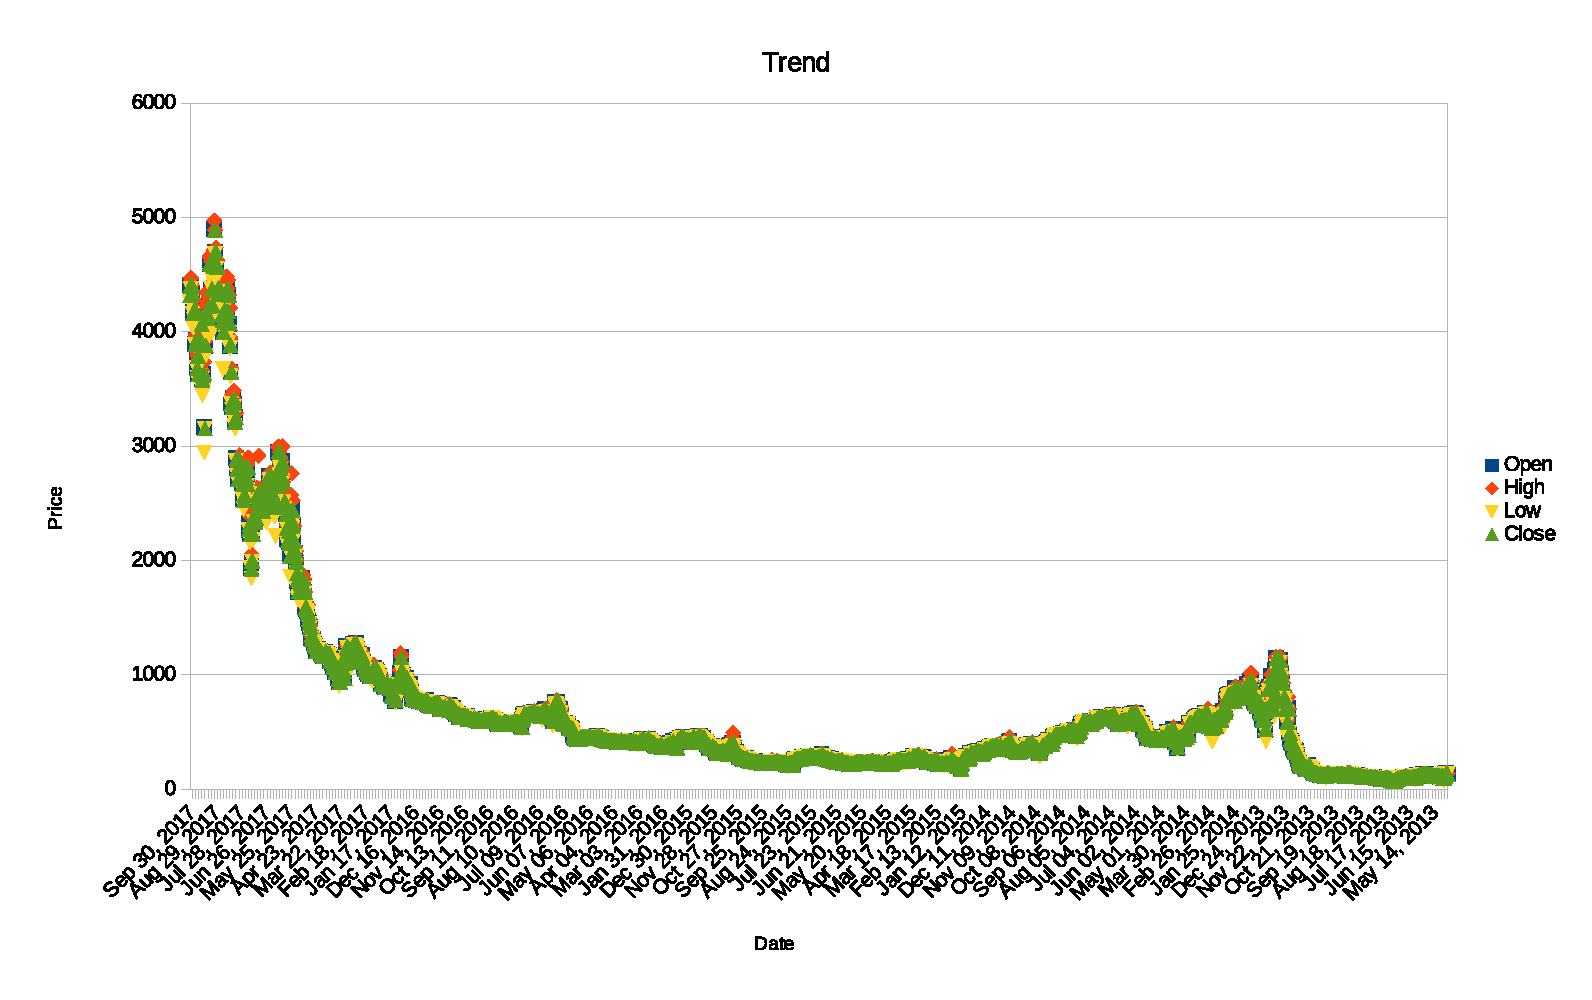
\includegraphics[width=\linewidth]{bitcoin_price_trend.eps}
    \caption{Daily Price Trend}
    \label{fig:my_label}
\end{figure}

This data can be used to:
\begin{itemize}
\item Predict cryptocurrency price in the future.

\item This also helps to analyse the surge in the market.

\item The comparision of this chart between different cryptocurrencies will help us to compare them and find the popular cryptocurrency and the one which has got the highest price.

We have also plotted the box plot and see there are lot of outliers, that is because there has been surge recently in crypto currency especially bitcoin trading activities.These outliers also help to analyse any anamolies. 

For a given continuous variable, outliers are those observations that lie outside 1.5 * IQR, where IQR, the ‘Inter Quartile Range’ is the difference between 75th and 25th quartiles. Look at the points outside the whiskers in below box plot.

\ Below figures show the Univariate approach(BoxPlot On single Column or Attribute)

Figure 2 captures ouliers for High Price for High for BitcoinPrice.csv. We are plotting only one column or attribute “High” present in the BitcoinPrice.csv

Figure 3 captures outliers for Market Price for BitCoin Dataset.csv.\newline

Bivariate Approach for Marking Outliers\newine
 
Figure 4 captures BoxPlot for Market Price and Market Cap for bitcoin datset.csv. We observe outliers which show up as dots.

Figure 5 BoxPlot for btc\textunderscore total\textunderscore bitcoins versus avg \textunderscore block\textunderscore size for bitcoin dataset.csv. We observe there are two outliers which show up as dots outside the whiskers of box plot.


\begin{figure}
    \centering
    \includegraphics[width=\linewidth]{High_Price}
    \caption{High \textunderscore Price}
    \label{fig:my_label}
\end{figure}




\begin{figure}
    \centering
    \includegraphics[width=\linewidth]{Bitcoin_Market_Price}
    \caption{Bitcoin\textunderscore Market\textunderscore Price\textunderscore Outliers}
    \label{fig:my_label}
\end{figure}


\begin{figure}
    \centering
    \includegraphics[width=\linewidth]{BitcoinMarketPriceandMarketCap}
    \caption{BitcoinMarketPriceandMarketCap Outlier}
    \label{fig:my_label}
\end{figure}


\begin{figure}
    \centering
    \includegraphics[width=\linewidth]{BoxplotforTotalBitcoinsandAvgBlockSize}
    \caption{BoxplotforTotalBitcoinsandAvgBlockSize}
    \label{fig:my_label}
\end{figure}


\end{itemize}


\section{Verify Data Quality}

Data has been verified to identify:

\begin{itemize}
\item 
Missing data: Using R, We identified that bitcoin price dataset has missing values for Volume for 7 months of Year 2013. It amounts to around 15\% of the data.
We also found that bitcoin dataset contains around 27 missing values, which was only around 0.92\% of the total dataset.

\item
Data Errors: The dataset is mostly numeric and so doesn't have any errors as such. Further there is no
text or factor data, so there are no typographical errors.

\item 
Measurement Errors: There is single source of data and is based on single measurement scheme, so there are no measurement errors recorded.

\item 
Coding inconsistencies: Since the data is from single source, there are no coding inconsistencies. Further we have single format of files i.e. csv, all follow the same delimiter scheme.

\item
Bad Metadata: Metadata is from standard terminology, so there were no bad metadata issues.
    
\end{itemize}

\section{Data Understanding}
\subsection{Selecting Data}

The data selected contains hand crafted features. Bitcoin\textunderscore Dataset has 24 features which describe various aspects of bitcoin. Also Bitcoin Price.csv has features like High Price, Low Price which helps us in determining Average Price based on these two 

\subsection{Data Cleaning}
\subsubsection{Missing Values}

There are following possible ways to handle missing values:
\begin{itemize}
    \item 
    Ignore the tuple: This method can be used when the percentage of missing data is very less. We have used this technique for handling missing data in bitcoin dataset as we had only 0.92\% of missing data.
    \item
    Fill in the missing value manually: Since this is time series data, this option is not possible.
    
    \item
    Use a global constant to fill the missing value: Again, since this is a time series data, a single global constant may not give the right value and affect the overall analysis.
    
    \item
    Use a measure of central tendency for the attribute(mean or median): Since this is time series data, further has very high volatility since cryptocurrency trading is comparatively very new, mean/median would result in biases.
    
    \item
    Use the attribute mean or median for all samples belonging to the same class: This mechanism can be used in context of time. We can fill the missing values with the average of its nearest set of time period, eg. weekly or monthly or yearly average. It can be decided to take monthly/yearly by analyzing the trend in the visual charts.
    
    \item
    Use the most probably value to fill in the missing value: This technique can also be used to predict the missing value based on its most correlated attribute. The correlated attribute can be identified based on domain knowledge or by plotting the charts. Since time\textunderscore series data is continuous data, we can use Linear Regression technique to predict the missing related value.
\end{itemize}

\textbf
{Handling Missing Values in Volume in bitcoin price data}


\begin{figure}
    \centering
    \includegraphics[width=\linewidth]{bitcoin_price_with_missing_values}
    \caption{Bitcoin Volume Against Date}
    \label{fig:my_label}
\end{figure}

Figure 2. shows that volume has been consistent across the whole year of 2014 with slight peaks.

We have used two ways to identify the missing values. After that we plotted again to verify our prediction.

1. From our domain information, we consider that volume of the price might get impacted based on its average daily price.\\

We calculate the average daily price by taking average of daily High and Low. Using linear regression model then we build a model between Volume and Average Daily Price. And then we predict the missing values for Volume based on respective average daily prices.\newline

\begin{figure}
    \centering
    \includegraphics[width=\linewidth]{AverageDailyPrice_Volume_AfterFillingMissing.png}
    \caption{Using Linear Regression}
    \label{fig:my_label}
\end{figure}

Figure 3 shows the chart with filled missing values using this method.
\newline
2. Looking at the Figure 2, it can be seen that the trend in volume of trading has been consistent across year 2014. So, we applied the method where we can take the mean of similar class and use that mean value to fill the missing values.
Thus, we calculate the mean for Dec 2013 to Dec 2014 and then use that mean to fill the missing value.
This will avoid any biases as we take the mean from the similar class and not overall.\\
\begin{figure}
    \centering
    \includegraphics[width=\linewidth]{Volume_After_Filling_Missing_Value.png}
    \caption{Using Nearest Neighbour Mean}
    \label{fig:my_label}
\end{figure}
Figure 4 shows the chart after filled missing values using this method.\newline
If we compare Figure 3 and Figure 4, we can see that in this particular case, regression mechanism
didn't predict the values so correctly, but using the mean from nearest neighbour was more consistent.\\

So, we go ahead with technique 2 and use that for filling our missing values.

\begin{figure}
    \centering
    \includegraphics[width=\linewidth]{MissingValue_Against_Date.png}
    \caption{Missing Values Against Date after Filling}
    \label{fig:my_label}
\end{figure}

Figure 5 shows that missing values are in trend after filling.\newline

\textbf{Handling missing values in the bitcoin\_dataset.}

Bitcoin Dataset has only 27 missing values, which amounted to around 0.92\% of the total dataset. Since this is very small amount and ignoring them may not impact the overall analysis, we used
the technique to ignore the missing values.\\

We thus clean the data by removing the rows with missing values.


\subsection{Construct Data}
\subsubsection{Derived Attributes}

bitcoin price dataset.

As we looked at the price dataset, we see there are Open, Close, High and Low attributes. However, there is one more attribute which can be useful in price prediction. And that is called average price.
Based on average price, Average price enables investor to decide to trade or not and might impact the
volume. However, if the volatility is very high, sometimes it may not give right prediction.

We have calculated average daily price using (Low + High)/2 for bitcoin dataset.


\subsection{Integrating and Formatting the Data}

We have applied different suitable R techniques and preprocessed the data appropriately.We have used R scripts for detecting outliers and visualizing the data in the form of Graphs.We have used R for Removing the missing Values and Normalizing the data. Linear Regression Techniques were also used. We have used Tableau for Visualizations for Bitcoin and Etherium Dataset. 

\end{document}